\section{Problem (1)}
	You drop an $11.2 \ lb$ book to a friend who stands on the ground at distance $D = 39.0 \ ft$ below. If your friend's outstretched hands are at distance $d = 5.3 \ ft$ above the ground:

	\begin{figure}[H]
		\begin{center}
			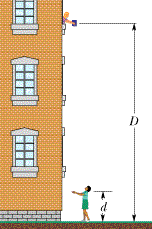
\includegraphics[scale=1]{hw8_problem1}
			\caption{Illustration of Problem 1}
			\label{fig:hw8_problem1}
		\end{center}
	\end{figure}

	\subsection{Question (a)}

		How much work $W_{g}$ does the gravitational force do on the book as it drops to her hands?

		\textbf{R:}

		\begin{align}
			W_{g} = \ &F_{g} \Delta y& \notag \\
			= \ &(11.2 \ lb) [(5.3 \ ft) - (39.0 \ ft)]& \notag \\
			= \ &- 377.44 \ ft \times lb&
		\end{align}

	\subsection{Question (b)}

		What is the change $\Delta U$ in the gravitational potential energy of the book-Earth system during the drop?

		\textbf{R:}

		\begin{align}
			\Delta U_{g} = \ &U_{g_{f}} - U_{g_{i}}& \notag \\
			= \ &mgy_{f} - mgy_{i}& \notag \\
			= \ &[(11.2 \ lb)(5.3 \ ft)] - [(11.2 \ lb)(39.0 \ ft)]& \notag \\
			= \ &(59.36 \ ft \times lb) - (436.8 \ ft \times lb)& \notag \\
			= \ &-377.44 \ ft \times lb&
		\end{align}
